\begin{figure}[htbp]
    \centering
    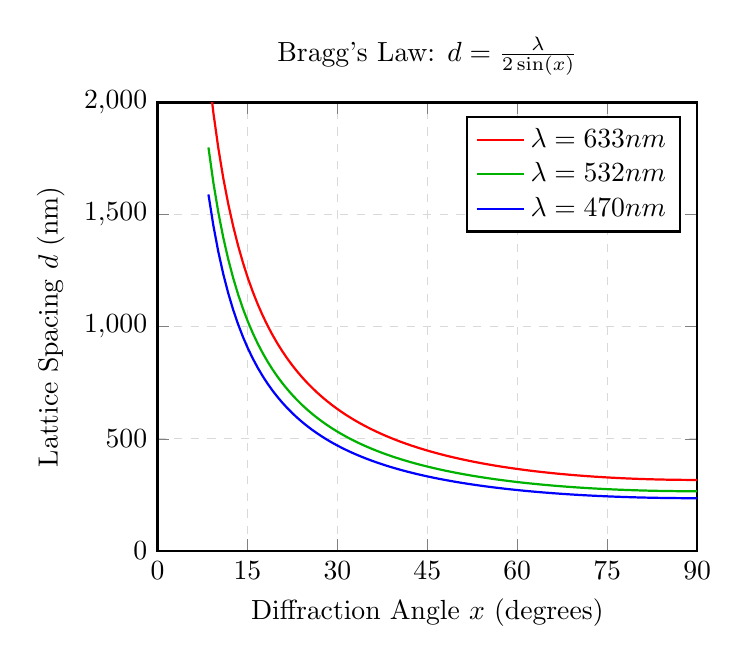
\begin{tikzpicture}
        \begin{axis}[
            title={Bragg's Law: $d = \frac{\lambda}{2 \sin(x)}$},
            xlabel={Diffraction Angle $x$ (degrees)},
            ylabel={Lattice Spacing $d$ (nm)},
            xmin=0, xmax=90,
            ymin=0, ymax=2000,
            xtick={0, 15, 30, 45, 60, 75, 90},
            ytick={0, 500, 1000, 1500, 2000},
            domain=8.5:90, % Keeps y values just under 2200 to prevent graph distortion
            samples=100,   % Number of points to sample for smooth curves
            grid=both,
            grid style={dashed, gray!30},
            restrict y to domain=0:2500, % Prevents calculation overflow near x=0
            thick,
            legend pos=north east % Positions the legend in the top right
        ]
            % 633 nm (Red light)
            \addplot [color=red, thick] {633 / (2 * sin(x))};
            \addlegendentry{$\lambda = 633 \text{ nm}$}
            
            % 532 nm (Green light)
            \addplot [color=green!70!black, thick] {532 / (2 * sin(x))};
            \addlegendentry{$\lambda = 532 \text{ nm}$}
            
            % 470 nm (Blue light)
            \addplot [color=blue, thick] {470 / (2 * sin(x))};
            \addlegendentry{$\lambda = 470 \text{ nm}$}
        \end{axis}
    \end{tikzpicture}
    \caption{Lattice spacing $d$ as a function of the diffraction angle $x$ for visible light wavelengths of $633 \text{ nm}$ (red), $532 \text{ nm}$ (green), and $470 \text{ nm}$ (blue).}
    \label{fig:braggs_law_multiple}
\end{figure}